\section{Le Code }
\label{sec:Ch1}

%%%%%%%%%%%%%%%%%%%%%%%%%%%%%%%%%%%% SUBSECTION 1
\subsection{Le cas d'étude - 2D} 
\label{sec:Ch1.1}

On étudie dans un premier temps La fonction de Breukels pour en chercher les optimum. On utilise pour ce faire un code d'optimsiation fournit par la bibliothèque \textbf{aerosandbox} et on se place dans le cas d'optimisation suivant: 
\begin{itemize}
    \item Maximum de $\sum_{\alpha = 0}^{20}\frac{C_L(\alpha)}{C_D(\alpha)} Gaussienne(alpha, center, sigma) $
\end{itemize}

    où $Gaussienne(\alpha, center, \sigma) = e^{-\frac{(center - \alpha)^2}{2\sigma^2}}$ est une Gaussienne permettant d'obtenir une moyenne pondérée. 

\underline{Les résultats sont présentés dans la partie suivante.}
\begin{figure}[H]
    \centering
    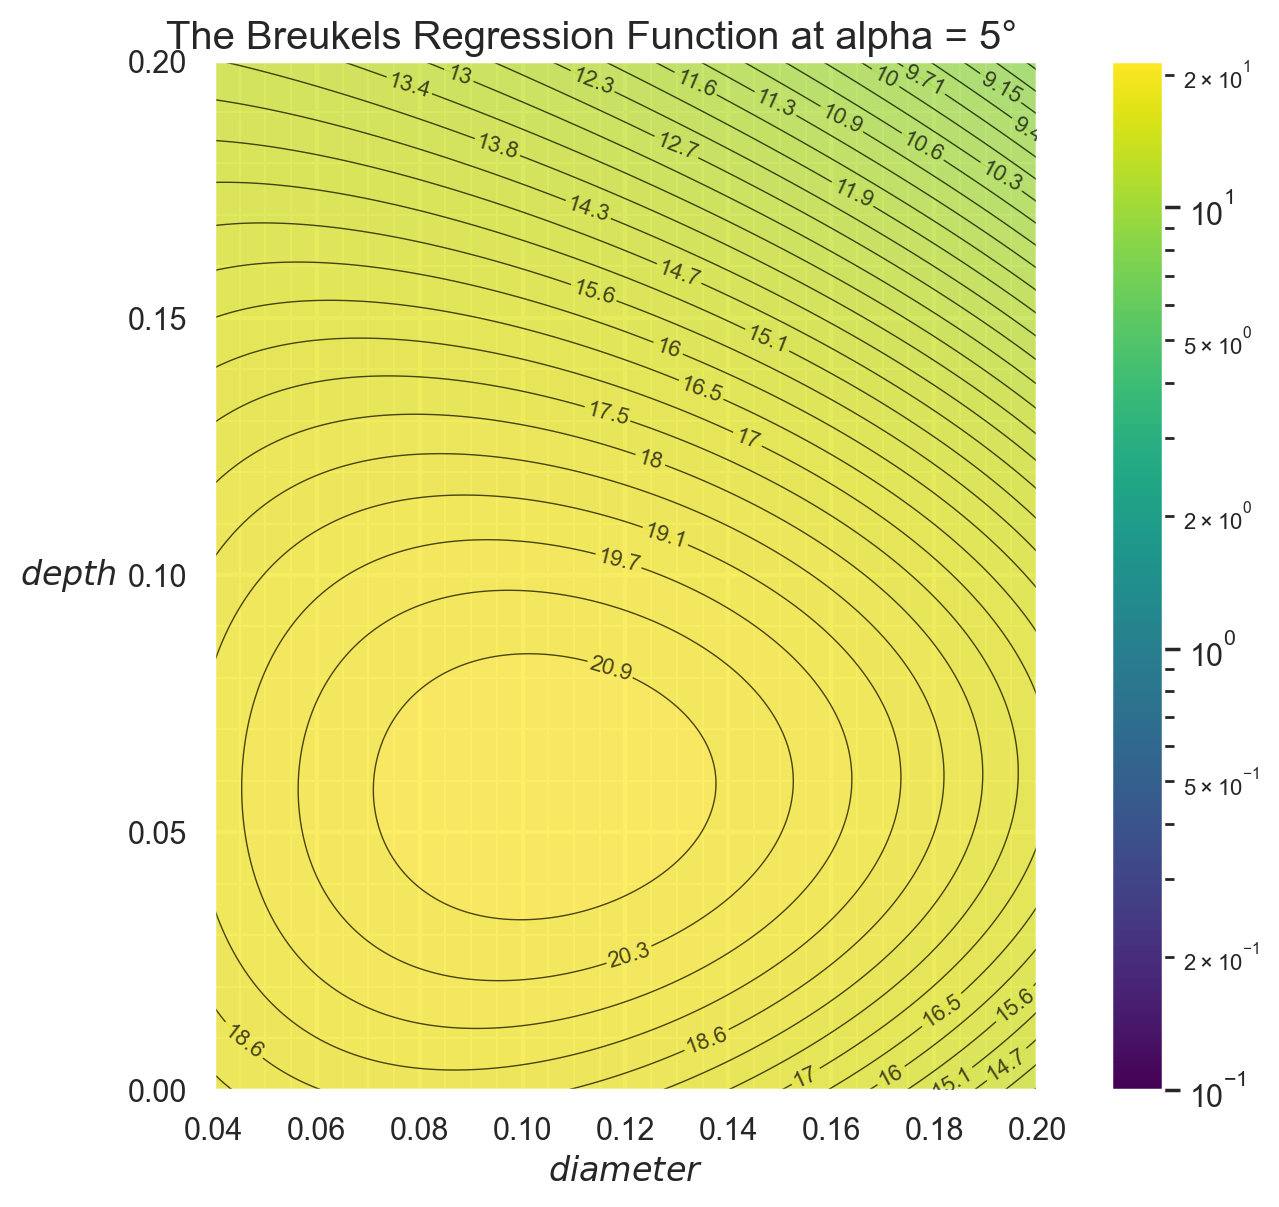
\includegraphics[width=0.5\textwidth]{Pics/breukels.png}  
    \caption{Tracer de $\frac{C_L}{C_D}$ par Régression de Breukels à $\alpha$=5°}
    \label{fig:breukels}
\end{figure}

%%%%%%%%%%%%%%%%%%%%%%%%%%%%%%%%%%%% SUBSECTION 2
\subsection{Le cas d'étude - 3D} 
\label{sec:Ch1.2}

\textbf{L'étude est réalisée à 50 knots}.\\
On se place dans le cas d'étude d'un SK50-VG dont on fait varier le \textbf{diamètre t entre -0.02 et +0.1 et la cambrure k entre -0.1 et 0.1}. \\
    
    On ajoute sur chaque rib les limites suivantes :
    \begin{itemize}
        \item \textbf{le diamètre ne peut pas être inférieur à 0.04}
        \item \textbf{la cambrure ne peut pas être inférieure au demi-diamètre}
    \end{itemize}

    Ainsi, les résultats sont à nuancer : \textbf{une aile avec un certain delta de t ou de k ne veut pas dire que toutes les sections ont été modifiées de ce delta; seules les sections respectant ces critères de minimum énoncés précédemment le sont.}

La loi d'évolution de t et k sur une VG est initialement:  
\begin{itemize}
    \item t : [0.07 0.067 0.065 0.063 0.061 0.06 0.06  0.06 0.06 0.06  0.06  0.06 0.06 0.06  0.06 0.061 0.063 0.065 0.067 0.07]
    \item k : [0.034 0.05 0.0645 0.0686 0.072 0.075 0.08 0.08 0.08 0.08      0.08 0.08 0.08 0.08 0.075 0.072 0.0686 0.0645 0.05 0.034]
\end{itemize}

    A nouveau, on cherche l'optimum dans le problème d'optimisation suivants:
    \begin{itemize}
        \item Maximum de $\sum_{\alpha = 0}^{21}\frac{C_L(\alpha)}{C_D(\alpha)} Gaussienne(alpha, center, sigma) $
    \end{itemize}
    \underline{Les résultats sont présentés dans la partie suivante.}

\begin{figure}[H]
    \centering
    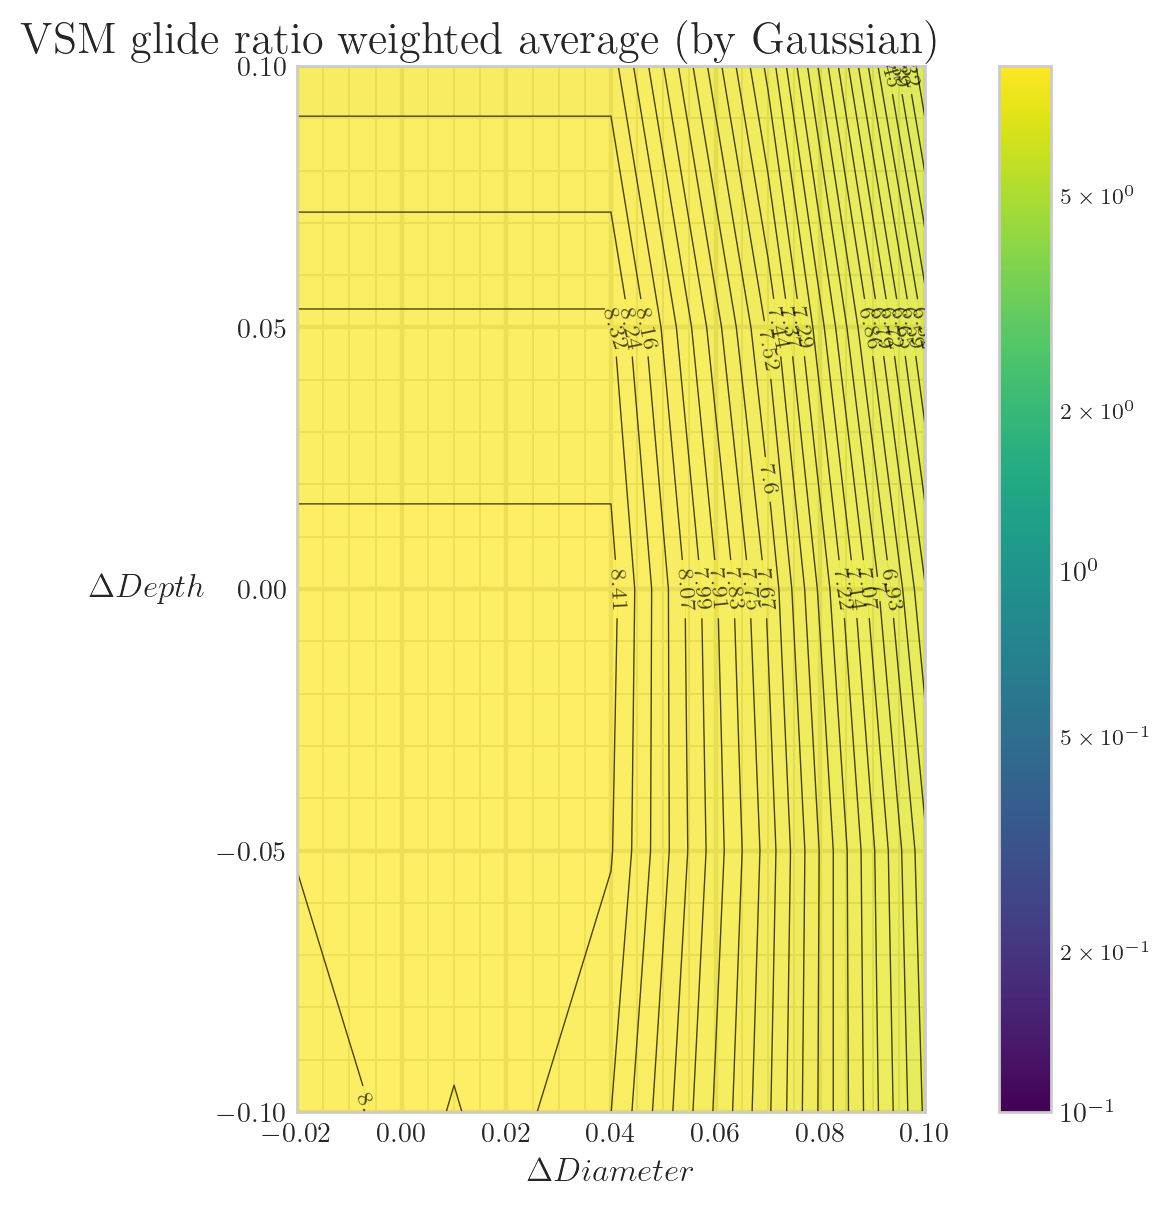
\includegraphics[width=0.5\textwidth]{Pics/vsm.png}  
    \caption{Tracer de $\frac{C_L}{C_D}$ par VSM en faisant varier (t,k)}
    \label{fig:vsm}
\end{figure}